% The short baseline neutrino detector
\section{Short Baseline Neutrino Program}

Understanding the anomalies observed at \gls{lsnd} and MiniBooNE is one of the goals of the proposed \gls{sbn} program.
The program includes three \glspl{lartpc} located along the \gls{bnb} at Fermilab: \gls{sbnd}, MicroBooNE and Icarus.
This section aims to give an overview of the \gls{sbn} program beam and detectors.

\subsection{The Booster Neutrino Beam line}
The \gls{bnb} is one of the neutrino sources from Fermilab's Accelerator Complex, which comprises seven particle accelerators and storage rings\marginnote{including the main injector, \gls{numi}, the Tevatron, \ldots}.
The \gls{bnb} has successfully been operated for already 12 years in both neutrino and anti-neutrino modes.
The fluxes are well understood, systematic uncertainties associated with the beam have also been determined\cite[-.5em]{Antonello:2015lea}.
See figure \ref{fig:sbnp} for an overview of the location of the accelerators, detectors and the \gls{bnb} axis.
\begin{figure}
  \makebox[\textwidth]{%
  \begin{tikzpicture}
    % Map
    \node (img) {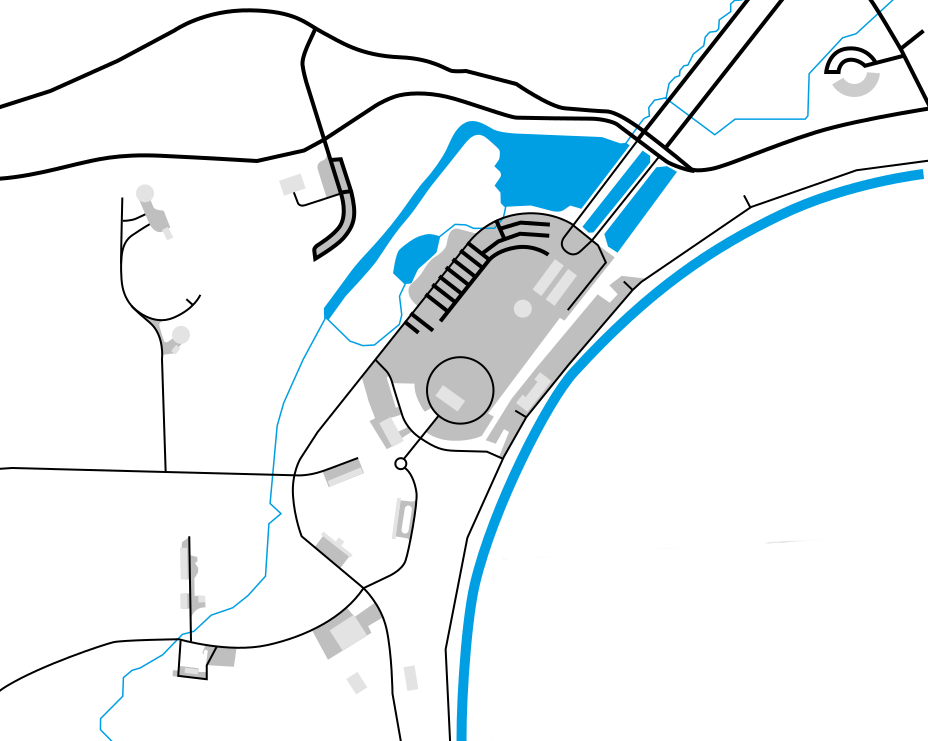
\includegraphics[width=\textwidth]{maps_fermilab_cutout}};
    % Accelerators
    \draw[solarized-red, very thick, densely dotted] ( -.05, -.225) circle (.4cm);
    \begin{scope}
      \clip(-6,-4.25) rectangle (3, 3);
      \begin{scope}[rotate=30]
        \draw[solarized-base0, very thick, densely dotted] (-5.9, -4.25) ellipse (2.6cm and 3.3cm);
      \end{scope}
    \end{scope}
    \draw[solarized-red, very thick, densely dashed] (-.45, -.225) -- (-.4, -1.55);
    \begin{scope}
      \clip(-2.4, -1.55) rectangle (2, -4);
      \draw[solarized-red, very thick, densely dashed] (-2.4, -1.55) circle (2cm);
    \end{scope}
    \begin{scope}
      \clip(-2.4, -2.8) rectangle (-4, -4);
      \draw[solarized-red, very thick, densely dashed] (-2.4, -2.8) circle (.75cm);
    \end{scope}
    % Target
    \draw[solarized-red,  very thick] (-3.15, -2.5) circle (.25cm);
    \draw (-3.15,-2.5) node[cross=.24cm, solarized-red, very thick] {};
    % Detectors
    \draw[solarized-blue, very thick] (-3.19, -1.7) circle (.2cm);
    \draw[solarized-magenta, very thick] (-3.3, .4) circle (.2cm);
    \draw[solarized-base0,very thick] (-3.3, .95) circle (.2cm);
    \draw[solarized-cyan,very thick] (-3.37, 1.3) circle (.2cm);
    \draw[solarized-base0,very thick,densely dashed] (-3.6, 1.9) circle (.3cm);
    % Beam lines
    \draw[solarized-blue, dashed, very thick, ->] (-3.175,-2.1) -- (-3.55, 4.2);
    \draw[solarized-base0, dashed, very thick, ->] (-1.5,-3.2) -- (-4.5,3.9);
    % Legende
    \draw[solarized-red, very thick, densely dotted] (1.5, -1)   circle (.15cm)
      node[anchor=west, inner sep=1em, black] {Booster Ring};
    \draw[solarized-red,very thick, densely dashed] (1.4, -1.6) -- (1.6, -1.4);
    \draw (1.5,-1.5) node[anchor=west, inner sep=1em, black] {Proton beam};
    \draw (1.5,-2) node[cross=.4em, solarized-red, very thick] {};
    \draw[solarized-red,  very thick] (1.5,-2) circle (.15cm)
      node[anchor=west, inner sep=1em, black] {Target \& decay pipe};
    \draw[solarized-blue,very thick, dashed, ->] (1.4, -2.6) -- (1.6, -2.4);
    \draw (1.5, -2.5) node[anchor=west, inner sep=1em, black] {\gls{bnb} axis};
    \draw[solarized-blue,   very thick] (1.5,-3.125)   circle (.15cm)
      node[anchor=west, inner sep=1em, black] {\gls{sbnd}};
    \draw[solarized-magenta, very thick] (1.5,-3.625) circle (.15cm)
      node[anchor=west, inner sep=1em, black] {MicroBooNE};
    \draw[solarized-cyan, very thick] (1.5,-4.125)   circle (.15cm)
      node[anchor=west, inner sep=1em, black] {Icarus};
  \end{tikzpicture}
  }
  \caption{%
    Traced map of Fermilab and the detectors involved in the \gls{sbn} program.
    The Main Injector, MiniBooNE, Minos, Minerva, Nova and the \gls{numi} axis were added as reference points.
  }
  \label{fig:sbnp}
\end{figure}

The beam's starting point is the radio-frequency quadrupole accelerator, which accelerates and separates the protons into bunches.
Then the protons pass through a 150m linear accelerator before they're fed to the Booster Ring.
After reaching energies of 8.89GeV in the ring the protons are guided to the beryllium target.
The target measures 71cm long\marginnote{The length of the target corresponds to 1.7 interaction lengths.} and is only 1cm in diameter.
The resulting charged particles are focused using a magnetic horn and decay in a 50m long region filled with air\marginnote{Commonly known as the decay pipe.}, where the \gls{bnb} is generated.
This region can be shortened to 25m with the use of an absorber to influence the resulting flux.

\subsection{MicroBooNe}

MicroBooNE is the first operative \gls{lartpc} detector of the \gls{sbn} program.
The observation of tracks started in August 2015 and the collaboration is already taking and registering data.
Figure \ref{fig:events_microboone} displays some neutrino event candidates observed at MicroBooNE.

\begin{figure}
  \centering
  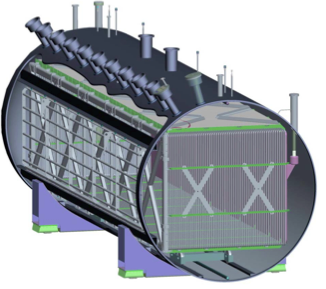
\includegraphics[width=.42\textwidth]{microboone_scheme}
  \caption{Scheme of the \gls{lartpc} of MicroBooNE}
  \label{fig:microboone_concept}
\end{figure}

MicroBooNE's active mass is 89 tons and its \gls{lartpc} is contained in a cryostat.
The active region is a rectangular volume of dimensions $2.33m \times 2.56m \times 10.37m$.
The cathode is situated at the boundary of the active volume on the left beam side of the detector.
The design of the chamber allows the ionization electrons of the charged particle tracks' to drift up to 2.56m to the wire grids, where the readout is made in the right beam side of the detector.
\Glspl{pmt} are installed behind the read out wire planes to collect prompt scintillation light produced in the argon.

\subsection{Short-Baseline Near Detector}

\begin{figure}
  \centering
  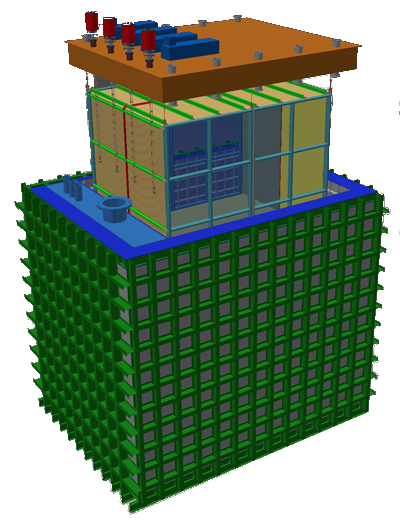
\includegraphics[width=.36\textwidth]{sbnd_detector_concept_new}
  \caption{Scheme of the \gls{sbnd}}
  \label{fig:sbnd_concept}
\end{figure}

The \gls{sbnd} is a \gls{lartpc} in contruction with an active volume of $4m \times 4m \times 5m$ at 110 meters from the \gls{bnb} target -- figure \ref{fig:sbnd_concept} illustrates its building concept.
The \gls{lartpc} has a capacity for 112 tons of liquid argon and is contained in a membrane-style cryostat.
It features four anode plane assemblies for signal readout.
The maximal drift distance of the ionization electrons is 2m, $\approx$20\% shorter than the maximal drift length in MicroBooNE.
\Gls{sbnd} will additionally feature a light collection system for detecting the scintillation light produced in the argon volume.
The operation of the \gls{sbnd} is planned to start in 2018.

